\documentclass[a4paper,11pt]{jarticle}

% レイアウト
\setlength{\hoffset}{0cm}
\setlength{\oddsidemargin}{-3mm}
\setlength{\evensidemargin}{-3cm}
\setlength{\marginparsep}{0cm}
\setlength{\marginparwidth}{0cm}
\setlength{\textheight}{24.7cm}
\setlength{\textwidth}{17cm}
\setlength{\topmargin}{-45pt}

\renewcommand{\baselinestretch}{1.2}
\renewcommand{\floatpagefraction}{1}
\renewcommand{\topfraction}{1}
\renewcommand{\bottomfraction}{1}
\renewcommand{\textfraction}{0}
\renewcommand\thefootnote{\arabic{footnote})}

% パッケージ
\usepackage[dvipdfmx]{graphicx}
\usepackage{amsmath,amssymb,epsfig}
\usepackage{eucal}
\usepackage{bm}
\usepackage{ascmac}
\usepackage{pifont}
\usepackage{multirow}
\usepackage{enumerate}
\usepackage{cases}
\usepackage{type1cm}
\usepackage{cancel}
\usepackage{url}
\usepackage{cite}
%\usepackage{color}
\usepackage[dvipdfmx]{color}
\usepackage{caption}
\usepackage[caption=false]{subfig}
\captionsetup[figure]{labelsep=space}
\usepackage{here}

% 擬似コード作成用
\usepackage[ruled,vlined]{algorithm2e}
\usepackage{setspace}
\DeclareRelationFont{JY1}{mc}{it}{}{OT1}{cmr}{it}{}
\DeclareRelationFont{JT1}{mc}{it}{}{OT1}{cmr}{it}{}
\DeclareFontShape{JY1}{mc}{m}{it}{<5> <6> <7> <8> <9> <10> sgen*min
    <10.95><12><14.4><17.28><20.74><24.88> min10
    <-> min10}{}
\DeclareFontShape{JT1}{mc}{m}{it}{<5> <6> <7> <8> <9> <10> sgen*tmin
    <10.95><12><14.4><17.28><20.74><24.88> tmin10
    <-> tmin10}{}
\DeclareRelationFont{JY1}{mc}{sl}{}{OT1}{cmr}{sl}{}
\DeclareRelationFont{JT1}{mc}{sl}{}{OT1}{cmr}{sl}{}
\DeclareFontShape{JY1}{mc}{m}{sl}{<5> <6> <7> <8> <9> <10> sgen*min
    <10.95><12><14.4><17.28><20.74><24.88> min10
    <-> min10}{}
\DeclareFontShape{JT1}{mc}{m}{sl}{<5> <6> <7> <8> <9> <10> sgen*tmin
    <10.95><12><14.4><17.28><20.74><24.88> tmin10
    <-> tmin10}{}
\DeclareRelationFont{JY1}{mc}{sc}{}{OT1}{cmr}{sc}{}
\DeclareRelationFont{JT1}{mc}{sc}{}{OT1}{cmr}{sc}{}
\DeclareFontShape{JY1}{mc}{m}{sc}{<5> <6> <7> <8> <9> <10> sgen*min
    <10.95><12><14.4><17.28><20.74><24.88> min10
    <-> min10}{}
\DeclareFontShape{JT1}{mc}{m}{sc}{<5> <6> <7> <8> <9> <10> sgen*tmin
    <10.95><12><14.4><17.28><20.74><24.88> tmin10
    <-> tmin10}{}
\DeclareRelationFont{JY1}{gt}{it}{}{OT1}{cmbx}{it}{}
\DeclareRelationFont{JT1}{gt}{it}{}{OT1}{cmbx}{it}{}
\DeclareFontShape{JY1}{mc}{bx}{it}{<5> <6> <7> <8> <9> <10> sgen*goth
    <10.95><12><14.4><17.28><20.74><24.88> goth10
    <-> goth10}{}
\DeclareFontShape{JT1}{mc}{bx}{it}{<5> <6> <7> <8> <9> <10> sgen*tgoth
    <10.95><12><14.4><17.28><20.74><24.88> tgoth10
    <-> tgoth10}{}
\DeclareRelationFont{JY1}{gt}{sl}{}{OT1}{cmbx}{sl}{}
\DeclareRelationFont{JT1}{gt}{sl}{}{OT1}{cmbx}{sl}{}
\DeclareFontShape{JY1}{mc}{bx}{sl}{<5> <6> <7> <8> <9> <10> sgen*goth
    <10.95><12><14.4><17.28><20.74><24.88> goth10
    <-> goth10}{}
\DeclareFontShape{JT1}{mc}{bx}{sl}{<5> <6> <7> <8> <9> <10> sgen*tgoth
    <10.95><12><14.4><17.28><20.74><24.88> tgoth10
    <-> tgoth10}{}
\DeclareRelationFont{JY1}{gt}{sc}{}{OT1}{cmbx}{sc}{}
\DeclareRelationFont{JT1}{gt}{sc}{}{OT1}{cmbx}{sc}{}
\DeclareFontShape{JY1}{mc}{bx}{sc}{<5> <6> <7> <8> <9> <10> sgen*goth
    <10.95><12><14.4><17.28><20.74><24.88> goth10
    <-> goth10}{}
\DeclareFontShape{JT1}{mc}{bx}{sc}{<5> <6> <7> <8> <9> <10> sgen*tgoth
    <10.95><12><14.4><17.28><20.74><24.88> tgoth10
    <-> tgoth10}{}
\DeclareRelationFont{JY1}{gt}{it}{}{OT1}{cmr}{it}{}
\DeclareRelationFont{JT1}{gt}{it}{}{OT1}{cmr}{it}{}
\DeclareFontShape{JY1}{gt}{m}{it}{<5> <6> <7> <8> <9> <10> sgen*goth
    <10.95><12><14.4><17.28><20.74><24.88> goth10
    <-> goth10}{}
\DeclareFontShape{JT1}{gt}{m}{it}{<5> <6> <7> <8> <9> <10> sgen*tgoth
    <10.95><12><14.4><17.28><20.74><24.88> tgoth10
    <-> tgoth10}{}
\endinput
%%%% end of jdummy.def

% カウンタの設定
\setcounter{section}{0}
\setcounter{subsection}{0}
\setcounter{subsubsection}{0}
\setcounter{equation}{0}

% キャプションの図をFigに変更
\renewcommand{\figurename}{Fig.}
\renewcommand{\tablename}{Tab.}

% 式番号を式(章番号.番号)に
\makeatletter
\renewcommand{\theequation}{\arabic{equation}}
\@addtoreset{equation}{section}
\makeatother

% タイトル部分
\title{\vspace{-20truemm}
{\normalsize \rightline{平成29年\ 7月\ 28日}}
{\large 制御系構成特論\\}
レポート課題2\\
\date{}
\vspace{-2truemm}}
\author{機械知能工学専攻 知能制御工学コース \hspace{3mm} 17344219 \ 二宮 悠二}
%-------------------------------------------------------
%-------------------------------------------------------
% ドキュメントの開始
%-------------------------------------------------------
\begin{document}
\parindent = 0pt % 字下げoff
% 表紙
\titlepage
\maketitle
%-------------------------------------------------------
% 問題
%-------------------------------------------------------
{\Large{\bf 問題}}
\vspace{2mm}
%-------------------------------------------------------
\begin{enumerate}
 \item ~~ $ G(s) = \dfrac{s-a}{(s-a)^2 + b^2} $において,$ x(0) = \left[ 0 ~~ - \frac{1}{b} \right]^T $のとき,入力$ u(t) = e^{at} $に対する応答$ y(t) $を求めよ.
 \item ~~ $ G_1 = \dfrac{s-1}{s+1} $,$ G_2 = \dfrac{1}{s-1} $の場合について,直列,並列結合を求め,結合後のシステムの可制御・可観測性を調べよ.またそれぞれにおいて結合後の伝達関数を求めよ.
 \item ~~ {\bf Fig.}{\ref{statability}}のフィードバック系で
  \begin{equation}
   P(s) = \dfrac{1}{s-1} , K(s) = \dfrac{s-1}{s} \nonumber
  \end{equation}
 としたとき,次のことを確かめよ.
  \begin{enumerate}[(1)]
   \setlength{\leftskip}{2mm}
   \item ~~ $ r $から$ y $までの伝達関数$ G_{yr}(s) $と$ d $から$ y $までの伝達関数$ G_{yd} (s) $を求め,それぞれの安定性を調べよ.
   \item ~~ (1) における2つの伝達関数の解析結果の相違点の原因は何かを述べよ.
   \item ~~ 特性方程式の極を調べ,閉ループ系の安定性を調べよ.
   \item ~~ $ P(s) $,$ K(s) $の実現を求め,閉ループ系の$ A $行列とその固有値を求めることで閉ループ系の安定性を調べよ.
   \item ~~ $ K(s) = \dfrac{3s+1}{s} $と変更したとき,フィードバック系の内部安定性を調べよ.
  \end{enumerate}
 \item ~~ あるシステムの実現
  \begin{center}
   $\left[
  \begin{array}{c|c}
   A & B \\ \hline
   C & D \\
  \end{array}
  \right] = \left[
  \begin{array}{cc|c}
   1 & 0 & 0 \\
   0 & -1 & 1 \\ \hline
   1 & 0 & 0 \\
  \end{array}
  \right]$
  \end{center}
 について,次の問に答えよ.
  \begin{enumerate}[(1)]
   \setlength{\leftskip}{2mm}
   \item システムの可制御・可観測性を調べよ.
   \item システムの可安定性・可検出性を調べよ.
  \end{enumerate}
\end{enumerate}
\newpage
\begin{figure}[t]
  \begin{center}
  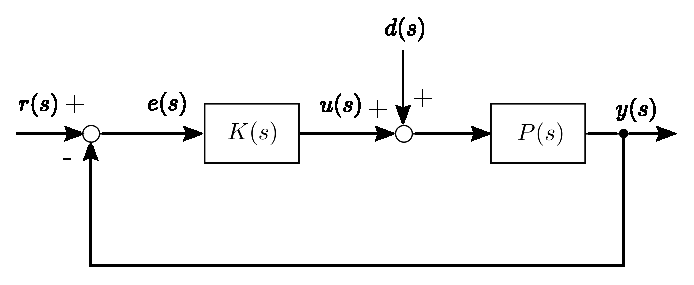
\includegraphics[scale=0.9]{../figure/eps/statability.eps}
  \caption{内部安定性}
  \label{statability}
 \end{center}
\end{figure}
%=======================================================
% 問1
%=======================================================
{\Large{\bf 解答}}
\vspace{2mm}
%=======================================================
\begin{enumerate}
 \item 
\ \ 伝達関数$ G(s) $は次のように変換できる.
\begin{equation*}
 G(s) = \left[
  \begin{array}{c|c}
   A & B \\ \hline
   C & D \\
  \end{array}
  \right] = \left[
  \begin{array}{cc|c}
   a & b & 1 \\
   -b & a & 0 \\ \hline
   1 & 0 & 0 \\
  \end{array}
  \right]
\end{equation*}
したがって
\begin{eqnarray*}
 y(s) & = & C (sI - A)^{-1} x(0) + C (sI - A)^{-1} B u(s)\\
      & = & [1 ~~ 0] \left[
		      \begin{array}{cc}
		       s-a & -b \\
		       b & s-a \\
		      \end{array}
		      \right]^{-1} \left[
		      \begin{array}{c}
		       0 \\
		       - \frac{1}{b} \\
		      \end{array}
				  \right] + [1 ~~ 0] \left[
				  \begin{array}{cc}
				   s-a & -b \\
				   b & s-a \\
				  \end{array}\right] \left[
				  \begin{array}{c}
				   1 \\
				   0 \\
				  \end{array}
						     \right] \cdot \dfrac{1}{s-a}\\
      & = & \dfrac{1}{(s-a)^2 + b^2}~ [~1 ~~ 0~] \left[
					      \begin{array}{cc}
					       s-a & b \\
					       -b & s-a \\
					      \end{array}
					      \right] \left[
						      \begin{array}{c}
						       0 \\
						       - \frac{1}{b} \\
						      \end{array}
						      \right] \nonumber \\
      &   & ~~~~ + \dfrac{1}{(s-a)^2 +b^2} ~ [~1 ~~ 0~] \left[
						     \begin{array}{cc}
						      s-a & b \\
						      -b & s-a \\
						     \end{array}
						    \right] \left[
						    \begin{array}{c}
						     1 \\
						     0 \\
						    \end{array}
							    \right] \cdot \dfrac{1}{s-a}\\
      & = & \dfrac{1}{(s-a)^2 + b^2} ~ [~ s-a ~~~ b ~] \left[
						\begin{array}{c}
						 0 \\
						 \ \frac{1}{b} \\
						\end{array}
						\right] + \dfrac{1}{(s-a)^2 +b^2} ~ [~s-a ~~~ b~] \left[
											     \begin{array}{c}
											      1 \\
											      0 \\
											     \end{array}
											     \right] \cdot \dfrac{1}{s-a}\\
      & = & \dfrac{1}{(s-a)^2 + b^2} ~ \cdot (-1) + \dfrac{1}{(s-a)^2 + b^2}\\\\
      & = & 0
\end{eqnarray*}
となる.よって入力信号が印加されても,出力信号は$ 0 $となり,入力は出力から遮断されていることが分かる.
%=======================================================
% 問2
%=======================================================
 \item \ \ それぞれのシステムをDoyleの記法を用いて表現することを考える.まず,$ G_1 $を状態空間表現すると
       \begin{eqnarray*}
	G_1 & = & \dfrac{s-1}{s+1}\\
	    & = & 1 + \dfrac{-2}{s+1}
       \end{eqnarray*}
       より,入出力の関係式は次のようになる.
       \begin{equation}
	y = \dfrac{-2}{s+1}u + u
       \end{equation}
       $ x = \dfrac{-2}{s+1}u $とおくと
       \begin{eqnarray*}
	x & = & \dfrac{-2}{s+1} u\\
	(s + 1)x & = & -2u\\
	\dot{x} & = & -x -2u
       \end{eqnarray*}
       より,状態方程式と出力方程式は次のようになる.
       \begin{eqnarray}
       	\begin{cases}
       	 \dot{x} = -x -2u & \\
       	 y = x + u &
       	\end{cases}
       \end{eqnarray}
       したがって
       \begin{eqnarray}
	G_1 & = & \left[
		   \begin{array}{c|c}
		    A_1 & B_1 \\ \hline
		     C_1 & D_1 \\
		   \end{array}\right] \nonumber \\
	    & = & \left[
		   \begin{array}{c|c}
		    -1 & -2 \\ \hline
		     1 & 1 \\
		   \end{array}\right]
       \end{eqnarray}
       を得る.同様に$ G_2 $について,$ x = \dfrac{1}{s-1}u $とおくと
       \begin{eqnarray*}
	x & = & \dfrac{1}{s-1}u\\
	(s-1)x & = & u\\
	\dot{x} & = & x + u
       \end{eqnarray*}
       より,状態方程式と出力方程式は次のようになる.
       \begin{eqnarray}
	\begin{cases}
	 \dot{x} = x + u &\\
	 y = x &
	\end{cases}
       \end{eqnarray}
       したがって
       \begin{eqnarray}
	G_2 & = & \left[
		  \begin{array}{c|c}
		   A_2 & B_2 \\ \hline
		   C_2 & D_2 \\
		  \end{array}\right] \nonumber \\
	    & = & \left[
		  \begin{array}{c|c}
		   1 & 1 \\ \hline
		   1 & 0 \\
		  \end{array}\right]
       \end{eqnarray}
       を得る.\\
       \ \ 直列結合の場合の伝達関数を$ G_c $とすると
       \begin{eqnarray}
	G_c & = & G_1 G_2 \nonumber \\
	  & = & \left[
		\begin{array}{cc|c}
		 A_1 & B_1 C_2 & B_1 D_2 \\
		 0 & A_2 & B_2 \\ \hline
		 C_1 & D_1 C_2 & D_1 D_2 \\
		\end{array}\right] \nonumber \\
	  & = & \left[
		\begin{array}{cc|c}
		 -1 & -2 & 0 \\
		 0 & 1 & 1 \\ \hline
		 1 & 1 & 0 \\
		\end{array}\right] \nonumber \\
	  & = & \left[
		\begin{array}{c|c}
		 A & B \\ \hline
		 C & D \\
		\end{array}\right]
       \end{eqnarray}
       と表せる.可制御性行列$ U_c $と可観測性行列$ U_o $の行列式がそれぞれ$ {\rm det} U_c \neq 0 $,$ {\rm det} U_o \neq 0 $を満たせば可制御,可観測である.
       \begin{eqnarray}
	{\rm det} U_c & = & {\rm det}\left[
			     \begin{array}{cc}
			      B & AB \\
			     \end{array}\right] \nonumber \\
	              & = & {\rm det}\left[
			     \begin{array}{cc}
			      0 & -2 \\
			      1 & 1 \\
			     \end{array}\right] \nonumber \\
	              & = & 2 \neq 0
       \end{eqnarray}
       \begin{eqnarray}
	{\rm det} U_o & = & {\rm det}\left[
				     \begin{array}{c}
				      C \\
				      CA \\
				     \end{array}\right] \nonumber \\
	              & = & {\rm det}\left[
				     \begin{array}{cc}
				      1 & 1 \\
				      -1 & -1 \\
				     \end{array}\right] \nonumber \\
	              & = & 0
       \end{eqnarray}
       \ \ 以上より,直列結合の場合システムは可制御,不可観測であり,このときの伝達関数$ G_c $は
       \begin{equation}
	G_c = \dfrac{1}{s+1}
       \end{equation}
       となる.
       \ \ 一方,並列結合の場合の伝達関数を$ G_p $とすると
       \begin{eqnarray}
	G_p & = & G_2 + G_2 \nonumber \\
	    & = & \left[
		\begin{array}{cc|c}
		 A_1 & 0 & B_1 \\
		 0 & A_2 & B_2 \\ \hline
		 C_1 & C_2 & D_1 + D_2 \\
		\end{array}\right] \nonumber \\
	    & = & \left[
		  \begin{array}{cc|c}
		   1 & 0 & 1 \\
		   0 & 1 & 1 \\ \hline
		   1 & 1 & 0 \\
		  \end{array}\right]
       \end{eqnarray}
       となる.このシステムの可制御性行列と可観測性行列の行列式の値はそれぞれ次のようになる.
       \begin{eqnarray}
	{\rm det}U_c & = & {\rm det} \left[
				     \begin{array}{cc}
				      1 & 1 \\
				      1 & 1 \\
				     \end{array}\right] \nonumber \\
	             & = & 0
       \end{eqnarray}
       \begin{eqnarray}
	{\rm det} U_o & = & {\rm det}\left[
				     \begin{array}{cc}
				      1 & 1 \\
				      1 & 1 \\
				     \end{array}\right] \nonumber \\
	              & = & 0
       \end{eqnarray}
       \ \ 以上より,並列結合の場合システムは不可制御,不可観測であり,このときの伝達関数$ G_p $は
       \begin{equation}
	G_p = \dfrac{2}{s-1}
       \end{equation}
       となる.
%=======================================================
% 問3
%=======================================================
 \item
  \begin{enumerate}[(1)]
   \setlength{\leftskip}{2mm}
%=======================================================
   \item \ \ {\bf Fig.}{\ref{statability}}より各入出力の関係を式で表すと次のようになる.
	 \begin{eqnarray}
	  e(s) & = & r(s) - y(s)\\
	  u(s) & = & K(s)~e(s)\\
	  y(s) & = & P(s) \bigl(~ u(s) + d(s) ~\bigr)
	 \end{eqnarray}
	 上記3つの式より
	 \begin{eqnarray}
	  y(s) & = & P(s) \bigl(~ u(s) + d(s) ~\bigr) \nonumber \\
	       & = & P(s) \Bigl( K(s) ~\bigl(~ r(s) - y(s) ~\bigr) + d(s) \Bigr) \nonumber \\
	  \Bigl( 1 + P(s)K(s) \Bigr) y(s) & = & P(s)K(s)r(s) + P(s)d(s) \nonumber \\
	  y(s) & = & \dfrac{P(s)K(s)}{1 + P(s)K(s)}r(s) + \dfrac{P(s)}{1 + P(s)K(s)}d(s)
	 \label{G(s)}
	 \end{eqnarray}
	 を得る.式(\ref{G(s)})より,$ G_{yr}(s) $と$ G_{yd}(s) $はそれぞれ次のようになる.
	 \begin{eqnarray}
	  G_{yr}(s) & = & \dfrac{P(s)K(s)}{1 + P(s)K(s)} \nonumber \\
	            & = & \dfrac{ \frac{1}{s-1} \cdot \frac{s-1}{s} }{ 1 + \frac{1}{s-1} \cdot \frac{s-1}{s} } \nonumber\\
	            & = & \dfrac{1}{s+1}
	  \label{Gyr}
	 \end{eqnarray}
	 \begin{eqnarray}
	  G_{yd}(s) & = & \dfrac{P(s)}{1 + P(s)K(s)} \nonumber \\
	            & = & \dfrac{ \frac{1}{s-1} }{ 1 + \frac{1}{s-1} \cdot \frac{s-1}{s} } \nonumber \\
	            & = & \dfrac{\frac{s}{s-1}}{s+1}
	  \label{Gyd}
	 \end{eqnarray}
	 \ \ ここで,式(\ref{Gyr})はすべての極が負であるため安定,式(\ref{Gyd})は非負の極を持つため不安定である.
%=======================================================
   \item \ \ 伝達関数$ G_{yr} $の分子の計算においては極零相殺が起こっているが,$ G_{yd} $の分子の計算においてはそれが起こっていない.すなわち,これらの解析結果に違いが出るのは極零相殺が生じているためである.
         %式(\ref{Gyr})では分子において極零相殺が起こっているため,非負の極が生じず安定となっている.
%=======================================================
   \item \ \ 式(\ref{Gyr}),式(\ref{Gyd})を,特性多項式を求めるために次のように変形する.
	 \begin{eqnarray}
	  G_{yr}(s) & = & \dfrac{P(s)K(s)}{1 + P(s)K(s)} \nonumber \\
	            & = & \dfrac{ \frac{1}{s-1} \cdot \frac{s-1}{s} }{ 1 + \frac{1}{s-1} \cdot \frac{s-1}{s} } \nonumber\\
	            & = & \dfrac{s-1}{s^2-1}
	  \label{Gyr2}
	 \end{eqnarray}
	 \begin{eqnarray}
	  G_{yd}(s) & = & \dfrac{P(s)}{1 + P(s)K(s)} \nonumber \\
	            & = & \dfrac{ \frac{1}{s-1} }{ 1 + \frac{1}{s-1} \cdot \frac{s-1}{s} } \nonumber\\
	            & = & \dfrac{s}{s^2-1}
	  \label{Gyr2}
	 \end{eqnarray}
	 したがって,特性多項式$ \Phi (s) $は次のようになる.
	 \begin{equation}
	  \Phi (s) = s^2 - 1
	 \end{equation}
	 特性方程式は
	 \begin{eqnarray*}
	  \Phi (s) & = & 0 \\
	  s^2 -1 & = & 0
	 \end{eqnarray*}
	 となり,これを解くと,$ s = \pm 1 $を得る.\\
	 \ \ 以上より,特性多項式の根の実部に非負であるものが含まれるため,閉ループ系は不安定である.
%=======================================================
   \item \ \ $ P(s) $,$ K(s) $それぞれの実現を$ G_P = \left[ A_1 , B_1 , C_1, D_1 \right] $,$ G_K = \left[ A_2, B_2, C_2, D_2 \right] $とする.入力を$ u $,出力を$ y $とおけば,システムの状態空間表現から実現は次のように求まる.まず,$ P(s) $について
	\begin{eqnarray*}
	 y & = & P(s)u \nonumber\\
	   & = & \dfrac{1}{s-1}u
	\end{eqnarray*}
	$ x = \dfrac{1}{s-1}u $とおくと
	\begin{eqnarray*}
	 (s-1) x & = & u \\
	 \dot{x} & = & x + u
	\end{eqnarray*}
	したがって状態方程式と出力方程式は
	\begin{eqnarray}
	 \begin{cases}
	  \dot{x} = x + u & \\
	  y = x &
	 \end{cases}
	\end{eqnarray}
	より
	\begin{eqnarray}
	 G_P & = & \left[ ~ A_1, ~ B_1, ~ C_1, ~ D_1 ~ \right] \nonumber\\
	     & = & \left[ ~ 1, ~ 1, ~ 1, ~ 0 ~ \right]
	\end{eqnarray}
	 を得る.同様に$ K(s) $について
	\begin{eqnarray*}
	 y & = & K(s)\\
	   & = & \dfrac{s-1}{s}u\\
	   & = & -\dfrac{1}{s}u + u
	\end{eqnarray*}
	$ x = -\dfrac{1}{s} $とおくと
	\begin{eqnarray*}
	 sx & = & -u\\
	 \dot{x} & = & -u
	\end{eqnarray*}
	したがって状態方程式と出力方程式は
	\begin{eqnarray}
	 \begin{cases}
	  \dot{x} = -u & \\
	  y = x + u &
	 \end{cases}
	\end{eqnarray}
	 より
	 \begin{eqnarray}
	  G_K & = & \left[ ~ A_2, ~ B_2, ~ C_2, ~ D_2 ~ \right] \nonumber\\
	      & = & \left[ ~ 0, -1, ~ 1, ~ 1 ~ \right]
	 \end{eqnarray}
	 を得る.\\
	 \ \ 以上より,この閉ループ系の$ A $行列は次のように表される.
	 \begin{eqnarray}
	  A & = & \left[
		   \begin{array}{cc}
		    A_1 - B_1D_2R^{-1}_{12}C_1 & -B_1R^{-1}{21}C_2 \\
		    B_2R^{-1}_{12}C_1 & A_2 - B_2D_1R^{-1}_{21}C_2 \\
		   \end{array}
		  \right] \nonumber\\
	    & = & \left[
		   \begin{array}{cc}
		    0 & -1 \\
		    -1 & 0 \\
		   \end{array}
		  \right]
	 \end{eqnarray}
	 ただし,$ R_{12} = I + D_1D_2 $,$ R_{21} = I + D_2D_1 $である.この行列の固有値$ \lambda $は
	 \begin{eqnarray*}
	  {\rm def} ~ \left[ ~ \lambda I - A ~ \right] & = & 0\\
	  {\rm def} ~ \left[
		       \begin{array}{cc}
			\lambda & 1 \\
			1 & \lambda \\
		       \end{array}
		      \right] & = & 0 \\
	  ( \lambda^2 - 1 ) & = & 0
	 \end{eqnarray*}
	 で表され,これを解くと
	 \begin{equation}
	  \lambda = \pm 1
	 \end{equation}
	 を得る.\\
	 \ \ この固有値が閉ループ系の極を表し,実部が非負のものを含んでいるため閉ループ系は不安定であることが分かる.
%=======================================================
   \item \ \ フィードバック系の内部安定性を調べるには特性方程式の根の符号を調べればよい.$ K(s) = \dfrac{3s+1}{s} $のときの特性多項式$ \Phi (s) $は次のようになる.
	 \begin{eqnarray*}
	  \Phi (s) & = & 1 + P(s)K(s)\\
	           & = & s(s-1) + (3s + 1) \\
	           & = & s^2 + 2s + 1 \\
	           & = & (s + 1)^2
	 \end{eqnarray*}
	 よって,特性方程式の解は次のように求まる.
	 \begin{eqnarray*}
	  \begin{array}{rcl}
	   1 + P(s)K(s) & = & 0\\
	   s(s-1) + (3s + 1) & = & 0\\
	   s^2 + 2s + 1 & = & 0\\
	   (s + 1)^2 & = & 0\\
	   s & = & -1 ~~ (重解)
	  \end{array}
	 \end{eqnarray*}
	 \ \ 以上より,すべての根の実部が負であるため,このときのフィードバック系は内部安定となる.
  \end{enumerate}
%=======================================================
% 問4
%=======================================================
 \item
  \begin{enumerate}[(1)]
   \setlength{\leftskip}{2mm}
%=======================================================
   \item \ \ このシステムの可制御性行列$ U_c $の行列式の値は
	 \begin{eqnarray}
	  {\rm det} U_c & = & {\rm det} \left[
				      \begin{array}{cc}
				       B & BA \\
				      \end{array}
				      \right] \nonumber \\
	              & = & {\rm det} \left[
				      \begin{array}{cc}
				       0 & 0 \\
				       1 & -1 \\
				      \end{array}
				      \right] \nonumber \\
	              & = & 0
	 \end{eqnarray}
	 となる.また,可観測性行列$ U_o $の行列式の値は
	 \begin{eqnarray}
	  {\rm det} U_o & = & {\rm det} \left[
					\begin{array}{c}
					 C \\
					 CA \\
					\end{array}
					\right] \nonumber \\
	                & = & {\rm det} \left[
					\begin{array}{cc}
					 1 & 0 \\
					 1 & 0 \\
					\end{array}
					\right] \nonumber \\
	                & = & 0
	 \end{eqnarray}
	 となる.\\
	 \ \ したがって,システムは不可制御,不可観測である.
%=======================================================
   \item \ \ 行列$ A $の固有値は
	 \begin{eqnarray*}
	  {\rm det} ( \lambda I - A ) & = & 0\\
	  {\rm def} \left[
		    \begin{array}{cc}
		     \lambda - 1 & 0 \\
		     0 & \lambda +1 \\
		    \end{array}
		    \right] & = & 0\\
	  ( \lambda -1 )( \lambda +1 ) & = & 0\\
	  \lambda & = & \pm1
	 \end{eqnarray*}
	 である.$ {\rm Re}( \lambda ) \geq 0 $に対して行列$ \left[ ~ A - \lambda I ~~ B ~\right] $のランクが行フルランクとなれば可安定,行列$ \left[ ~ A - \lambda I ~~ C ~\right]^T $のランクが列フルランクとなれば可検出であるので,$ \lambda = 1 $として解析を行う.\\
	 \ \ まず,可安定性について考える.
	 \begin{eqnarray*}
	  \left[ ~ A - \lambda I ~~ B ~ \right] & = & \left[
						  \begin{array}{ccc}
						   1 - \lambda & 0 & 0\\
						   0 & -1-\lambda & 1\\
						  \end{array}
						  \right]\\
	                                        & = & \left[
						      \begin{array}{ccc}
						       0 & 0 & 0 \\
						       0 & -2 & 1 \\
						      \end{array}\right]
	 \end{eqnarray*}
	 この行列を行基本変形すると次のようになる.
	 \begin{eqnarray*}
	  \left[ ~ A - \lambda I ~~ B ~ \right] & → & \left[
						      \begin{array}{ccc}
						       0 & -2 & 1 \\
						       0 & 0 & 0 \\
						      \end{array}\right]
	 \end{eqnarray*}
	 したがって,$ {\rm rank} \left[ ~ A - \lambda ~~ B ~ \right] = 1 $であり,行フルランクではない.\\
	 \ \ 次に,可検出性について考える.
	 \begin{eqnarray*}
	  \left[
	  \begin{array}{c}
	   A - \lambda I \\
	   C \\
	  \end{array}
	  \right] & = & \left[
			\begin{array}{cc}
			 1 - \lambda & 0 \\
			 0 & -1 - \lambda \\
			 1 & 0 \\
			\end{array}\right]\\
	          & = & \left[
			 \begin{array}{cc}
			  0 & 0 \\
			  0 & -2 \\
			  1 & 0 \\
			 \end{array}\right]
	 \end{eqnarray*}
	 この行列を列基本変形すると次のようになる.
	 \begin{eqnarray*}
	  \left[
	  \begin{array}{c}
	   A - \lambda I \\
	   C \\
	  \end{array}\right] & → & \left[
				   \begin{array}{cc}
				    0 & 0 \\
				    0 & 1 \\
				    1 & 0 \\
				   \end{array}\right]
	 \end{eqnarray*}
	 したがって,$ {\rm rank} \left[ ~ A - \lambda I ~~ C ~ \right]^T = 2 $であり,列フルランクになる.\\
	 \ \ 以上より,このシステムは不可安定,可検出である.
  \end{enumerate}
%=======================================================
%=======================================================
\end{enumerate}
%=======================================================
%=======================================================
%=======================================================
%=======================================================
\end{document}
